% Created by tikzDevice version 0.12.3.1 on 2021-02-12 18:55:38
% !TEX encoding = UTF-8 Unicode
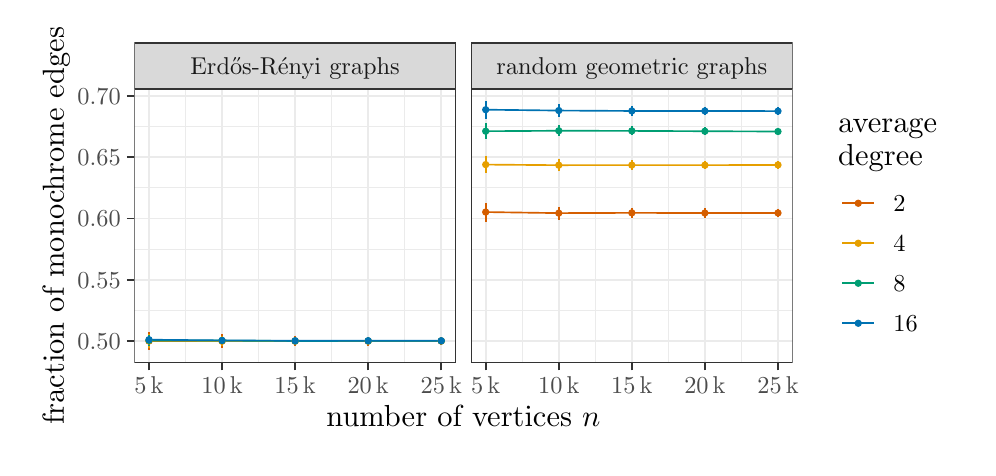
\begin{tikzpicture}[x=1pt,y=1pt]
\definecolor{fillColor}{RGB}{255,255,255}
\path[use as bounding box,fill=fillColor,fill opacity=0.00] (0,0) rectangle (339.67,151.77);
\begin{scope}
\path[clip] (  0.00,  0.00) rectangle (339.67,151.77);
\definecolor{drawColor}{RGB}{255,255,255}
\definecolor{fillColor}{RGB}{255,255,255}

\path[draw=drawColor,line width= 0.6pt,line join=round,line cap=round,fill=fillColor] (  0.00,  0.00) rectangle (339.67,151.77);
\end{scope}
\begin{scope}
\path[clip] ( 38.56, 30.69) rectangle (154.73,129.70);
\definecolor{fillColor}{RGB}{255,255,255}

\path[fill=fillColor] ( 38.56, 30.69) rectangle (154.73,129.70);
\definecolor{drawColor}{gray}{0.92}

\path[draw=drawColor,line width= 0.3pt,line join=round] ( 38.56, 49.62) --
	(154.73, 49.62);

\path[draw=drawColor,line width= 0.3pt,line join=round] ( 38.56, 71.78) --
	(154.73, 71.78);

\path[draw=drawColor,line width= 0.3pt,line join=round] ( 38.56, 93.93) --
	(154.73, 93.93);

\path[draw=drawColor,line width= 0.3pt,line join=round] ( 38.56,116.09) --
	(154.73,116.09);

\path[draw=drawColor,line width= 0.3pt,line join=round] ( 57.04, 30.69) --
	( 57.04,129.70);

\path[draw=drawColor,line width= 0.3pt,line join=round] ( 83.44, 30.69) --
	( 83.44,129.70);

\path[draw=drawColor,line width= 0.3pt,line join=round] (109.84, 30.69) --
	(109.84,129.70);

\path[draw=drawColor,line width= 0.3pt,line join=round] (136.24, 30.69) --
	(136.24,129.70);

\path[draw=drawColor,line width= 0.6pt,line join=round] ( 38.56, 38.55) --
	(154.73, 38.55);

\path[draw=drawColor,line width= 0.6pt,line join=round] ( 38.56, 60.70) --
	(154.73, 60.70);

\path[draw=drawColor,line width= 0.6pt,line join=round] ( 38.56, 82.86) --
	(154.73, 82.86);

\path[draw=drawColor,line width= 0.6pt,line join=round] ( 38.56,105.01) --
	(154.73,105.01);

\path[draw=drawColor,line width= 0.6pt,line join=round] ( 38.56,127.17) --
	(154.73,127.17);

\path[draw=drawColor,line width= 0.6pt,line join=round] ( 43.84, 30.69) --
	( 43.84,129.70);

\path[draw=drawColor,line width= 0.6pt,line join=round] ( 70.24, 30.69) --
	( 70.24,129.70);

\path[draw=drawColor,line width= 0.6pt,line join=round] ( 96.64, 30.69) --
	( 96.64,129.70);

\path[draw=drawColor,line width= 0.6pt,line join=round] (123.04, 30.69) --
	(123.04,129.70);

\path[draw=drawColor,line width= 0.6pt,line join=round] (149.45, 30.69) --
	(149.45,129.70);
\definecolor{drawColor}{RGB}{213,94,0}

\path[draw=drawColor,line width= 0.6pt,line join=round] ( 43.84, 41.78) --
	( 43.84, 41.78);

\path[draw=drawColor,line width= 0.6pt,line join=round] ( 43.84, 41.78) --
	( 43.84, 35.19);

\path[draw=drawColor,line width= 0.6pt,line join=round] ( 43.84, 35.19) --
	( 43.84, 35.19);

\path[draw=drawColor,line width= 0.6pt,line join=round] ( 70.24, 40.95) --
	( 70.24, 40.95);

\path[draw=drawColor,line width= 0.6pt,line join=round] ( 70.24, 40.95) --
	( 70.24, 36.19);

\path[draw=drawColor,line width= 0.6pt,line join=round] ( 70.24, 36.19) --
	( 70.24, 36.19);

\path[draw=drawColor,line width= 0.6pt,line join=round] ( 96.64, 40.47) --
	( 96.64, 40.47);

\path[draw=drawColor,line width= 0.6pt,line join=round] ( 96.64, 40.47) --
	( 96.64, 36.72);

\path[draw=drawColor,line width= 0.6pt,line join=round] ( 96.64, 36.72) --
	( 96.64, 36.72);

\path[draw=drawColor,line width= 0.6pt,line join=round] (123.04, 40.03) --
	(123.04, 40.03);

\path[draw=drawColor,line width= 0.6pt,line join=round] (123.04, 40.03) --
	(123.04, 36.92);

\path[draw=drawColor,line width= 0.6pt,line join=round] (123.04, 36.92) --
	(123.04, 36.92);

\path[draw=drawColor,line width= 0.6pt,line join=round] (149.45, 39.95) --
	(149.45, 39.95);

\path[draw=drawColor,line width= 0.6pt,line join=round] (149.45, 39.95) --
	(149.45, 37.08);

\path[draw=drawColor,line width= 0.6pt,line join=round] (149.45, 37.08) --
	(149.45, 37.08);
\definecolor{drawColor}{RGB}{230,159,0}

\path[draw=drawColor,line width= 0.6pt,line join=round] ( 43.84, 41.12) --
	( 43.84, 41.12);

\path[draw=drawColor,line width= 0.6pt,line join=round] ( 43.84, 41.12) --
	( 43.84, 36.02);

\path[draw=drawColor,line width= 0.6pt,line join=round] ( 43.84, 36.02) --
	( 43.84, 36.02);

\path[draw=drawColor,line width= 0.6pt,line join=round] ( 70.24, 40.30) --
	( 70.24, 40.30);

\path[draw=drawColor,line width= 0.6pt,line join=round] ( 70.24, 40.30) --
	( 70.24, 36.87);

\path[draw=drawColor,line width= 0.6pt,line join=round] ( 70.24, 36.87) --
	( 70.24, 36.87);

\path[draw=drawColor,line width= 0.6pt,line join=round] ( 96.64, 40.06) --
	( 96.64, 40.06);

\path[draw=drawColor,line width= 0.6pt,line join=round] ( 96.64, 40.06) --
	( 96.64, 37.09);

\path[draw=drawColor,line width= 0.6pt,line join=round] ( 96.64, 37.09) --
	( 96.64, 37.09);

\path[draw=drawColor,line width= 0.6pt,line join=round] (123.04, 39.77) --
	(123.04, 39.77);

\path[draw=drawColor,line width= 0.6pt,line join=round] (123.04, 39.77) --
	(123.04, 37.28);

\path[draw=drawColor,line width= 0.6pt,line join=round] (123.04, 37.28) --
	(123.04, 37.28);

\path[draw=drawColor,line width= 0.6pt,line join=round] (149.45, 39.66) --
	(149.45, 39.66);

\path[draw=drawColor,line width= 0.6pt,line join=round] (149.45, 39.66) --
	(149.45, 37.56);

\path[draw=drawColor,line width= 0.6pt,line join=round] (149.45, 37.56) --
	(149.45, 37.56);
\definecolor{drawColor}{RGB}{0,158,115}

\path[draw=drawColor,line width= 0.6pt,line join=round] ( 43.84, 40.66) --
	( 43.84, 40.66);

\path[draw=drawColor,line width= 0.6pt,line join=round] ( 43.84, 40.66) --
	( 43.84, 36.82);

\path[draw=drawColor,line width= 0.6pt,line join=round] ( 43.84, 36.82) --
	( 43.84, 36.82);

\path[draw=drawColor,line width= 0.6pt,line join=round] ( 70.24, 39.94) --
	( 70.24, 39.94);

\path[draw=drawColor,line width= 0.6pt,line join=round] ( 70.24, 39.94) --
	( 70.24, 37.44);

\path[draw=drawColor,line width= 0.6pt,line join=round] ( 70.24, 37.44) --
	( 70.24, 37.44);

\path[draw=drawColor,line width= 0.6pt,line join=round] ( 96.64, 39.69) --
	( 96.64, 39.69);

\path[draw=drawColor,line width= 0.6pt,line join=round] ( 96.64, 39.69) --
	( 96.64, 37.59);

\path[draw=drawColor,line width= 0.6pt,line join=round] ( 96.64, 37.59) --
	( 96.64, 37.59);

\path[draw=drawColor,line width= 0.6pt,line join=round] (123.04, 39.44) --
	(123.04, 39.44);

\path[draw=drawColor,line width= 0.6pt,line join=round] (123.04, 39.44) --
	(123.04, 37.74);

\path[draw=drawColor,line width= 0.6pt,line join=round] (123.04, 37.74) --
	(123.04, 37.74);

\path[draw=drawColor,line width= 0.6pt,line join=round] (149.45, 39.44) --
	(149.45, 39.44);

\path[draw=drawColor,line width= 0.6pt,line join=round] (149.45, 39.44) --
	(149.45, 37.75);

\path[draw=drawColor,line width= 0.6pt,line join=round] (149.45, 37.75) --
	(149.45, 37.75);
\definecolor{drawColor}{RGB}{0,114,178}

\path[draw=drawColor,line width= 0.6pt,line join=round] ( 43.84, 40.29) --
	( 43.84, 40.29);

\path[draw=drawColor,line width= 0.6pt,line join=round] ( 43.84, 40.29) --
	( 43.84, 37.66);

\path[draw=drawColor,line width= 0.6pt,line join=round] ( 43.84, 37.66) --
	( 43.84, 37.66);

\path[draw=drawColor,line width= 0.6pt,line join=round] ( 70.24, 39.65) --
	( 70.24, 39.65);

\path[draw=drawColor,line width= 0.6pt,line join=round] ( 70.24, 39.65) --
	( 70.24, 37.85);

\path[draw=drawColor,line width= 0.6pt,line join=round] ( 70.24, 37.85) --
	( 70.24, 37.85);

\path[draw=drawColor,line width= 0.6pt,line join=round] ( 96.64, 39.47) --
	( 96.64, 39.47);

\path[draw=drawColor,line width= 0.6pt,line join=round] ( 96.64, 39.47) --
	( 96.64, 37.83);

\path[draw=drawColor,line width= 0.6pt,line join=round] ( 96.64, 37.83) --
	( 96.64, 37.83);

\path[draw=drawColor,line width= 0.6pt,line join=round] (123.04, 39.32) --
	(123.04, 39.32);

\path[draw=drawColor,line width= 0.6pt,line join=round] (123.04, 39.32) --
	(123.04, 38.00);

\path[draw=drawColor,line width= 0.6pt,line join=round] (123.04, 38.00) --
	(123.04, 38.00);

\path[draw=drawColor,line width= 0.6pt,line join=round] (149.45, 39.22) --
	(149.45, 39.22);

\path[draw=drawColor,line width= 0.6pt,line join=round] (149.45, 39.22) --
	(149.45, 38.06);

\path[draw=drawColor,line width= 0.6pt,line join=round] (149.45, 38.06) --
	(149.45, 38.06);
\definecolor{drawColor}{RGB}{213,94,0}

\path[draw=drawColor,line width= 0.6pt,line join=round] ( 43.84, 38.53) --
	( 70.24, 38.49) --
	( 96.64, 38.49) --
	(123.04, 38.49) --
	(149.45, 38.54);
\definecolor{drawColor}{RGB}{230,159,0}

\path[draw=drawColor,line width= 0.6pt,line join=round] ( 43.84, 38.65) --
	( 70.24, 38.54) --
	( 96.64, 38.56) --
	(123.04, 38.56) --
	(149.45, 38.57);
\definecolor{drawColor}{RGB}{0,158,115}

\path[draw=drawColor,line width= 0.6pt,line join=round] ( 43.84, 38.76) --
	( 70.24, 38.71) --
	( 96.64, 38.56) --
	(123.04, 38.59) --
	(149.45, 38.59);
\definecolor{drawColor}{RGB}{0,114,178}

\path[draw=drawColor,line width= 0.6pt,line join=round] ( 43.84, 39.02) --
	( 70.24, 38.76) --
	( 96.64, 38.63) --
	(123.04, 38.65) --
	(149.45, 38.63);
\definecolor{drawColor}{RGB}{213,94,0}
\definecolor{fillColor}{RGB}{213,94,0}

\path[draw=drawColor,line width= 0.4pt,line join=round,line cap=round,fill=fillColor] ( 43.84, 38.53) circle (  1.11);

\path[draw=drawColor,line width= 0.4pt,line join=round,line cap=round,fill=fillColor] ( 70.24, 38.49) circle (  1.11);

\path[draw=drawColor,line width= 0.4pt,line join=round,line cap=round,fill=fillColor] ( 96.64, 38.49) circle (  1.11);

\path[draw=drawColor,line width= 0.4pt,line join=round,line cap=round,fill=fillColor] (123.04, 38.49) circle (  1.11);

\path[draw=drawColor,line width= 0.4pt,line join=round,line cap=round,fill=fillColor] (149.45, 38.54) circle (  1.11);
\definecolor{drawColor}{RGB}{230,159,0}
\definecolor{fillColor}{RGB}{230,159,0}

\path[draw=drawColor,line width= 0.4pt,line join=round,line cap=round,fill=fillColor] ( 43.84, 38.65) circle (  1.11);

\path[draw=drawColor,line width= 0.4pt,line join=round,line cap=round,fill=fillColor] ( 70.24, 38.54) circle (  1.11);

\path[draw=drawColor,line width= 0.4pt,line join=round,line cap=round,fill=fillColor] ( 96.64, 38.56) circle (  1.11);

\path[draw=drawColor,line width= 0.4pt,line join=round,line cap=round,fill=fillColor] (123.04, 38.56) circle (  1.11);

\path[draw=drawColor,line width= 0.4pt,line join=round,line cap=round,fill=fillColor] (149.45, 38.57) circle (  1.11);
\definecolor{drawColor}{RGB}{0,158,115}
\definecolor{fillColor}{RGB}{0,158,115}

\path[draw=drawColor,line width= 0.4pt,line join=round,line cap=round,fill=fillColor] ( 43.84, 38.76) circle (  1.11);

\path[draw=drawColor,line width= 0.4pt,line join=round,line cap=round,fill=fillColor] ( 70.24, 38.71) circle (  1.11);

\path[draw=drawColor,line width= 0.4pt,line join=round,line cap=round,fill=fillColor] ( 96.64, 38.56) circle (  1.11);

\path[draw=drawColor,line width= 0.4pt,line join=round,line cap=round,fill=fillColor] (123.04, 38.59) circle (  1.11);

\path[draw=drawColor,line width= 0.4pt,line join=round,line cap=round,fill=fillColor] (149.45, 38.59) circle (  1.11);
\definecolor{drawColor}{RGB}{0,114,178}
\definecolor{fillColor}{RGB}{0,114,178}

\path[draw=drawColor,line width= 0.4pt,line join=round,line cap=round,fill=fillColor] ( 43.84, 39.02) circle (  1.11);

\path[draw=drawColor,line width= 0.4pt,line join=round,line cap=round,fill=fillColor] ( 70.24, 38.76) circle (  1.11);

\path[draw=drawColor,line width= 0.4pt,line join=round,line cap=round,fill=fillColor] ( 96.64, 38.63) circle (  1.11);

\path[draw=drawColor,line width= 0.4pt,line join=round,line cap=round,fill=fillColor] (123.04, 38.65) circle (  1.11);

\path[draw=drawColor,line width= 0.4pt,line join=round,line cap=round,fill=fillColor] (149.45, 38.63) circle (  1.11);
\definecolor{drawColor}{gray}{0.20}

\path[draw=drawColor,line width= 0.6pt,line join=round,line cap=round] ( 38.56, 30.69) rectangle (154.73,129.70);
\end{scope}
\begin{scope}
\path[clip] (160.23, 30.69) rectangle (276.40,129.70);
\definecolor{fillColor}{RGB}{255,255,255}

\path[fill=fillColor] (160.23, 30.69) rectangle (276.40,129.70);
\definecolor{drawColor}{gray}{0.92}

\path[draw=drawColor,line width= 0.3pt,line join=round] (160.23, 49.62) --
	(276.40, 49.62);

\path[draw=drawColor,line width= 0.3pt,line join=round] (160.23, 71.78) --
	(276.40, 71.78);

\path[draw=drawColor,line width= 0.3pt,line join=round] (160.23, 93.93) --
	(276.40, 93.93);

\path[draw=drawColor,line width= 0.3pt,line join=round] (160.23,116.09) --
	(276.40,116.09);

\path[draw=drawColor,line width= 0.3pt,line join=round] (178.71, 30.69) --
	(178.71,129.70);

\path[draw=drawColor,line width= 0.3pt,line join=round] (205.11, 30.69) --
	(205.11,129.70);

\path[draw=drawColor,line width= 0.3pt,line join=round] (231.51, 30.69) --
	(231.51,129.70);

\path[draw=drawColor,line width= 0.3pt,line join=round] (257.92, 30.69) --
	(257.92,129.70);

\path[draw=drawColor,line width= 0.6pt,line join=round] (160.23, 38.55) --
	(276.40, 38.55);

\path[draw=drawColor,line width= 0.6pt,line join=round] (160.23, 60.70) --
	(276.40, 60.70);

\path[draw=drawColor,line width= 0.6pt,line join=round] (160.23, 82.86) --
	(276.40, 82.86);

\path[draw=drawColor,line width= 0.6pt,line join=round] (160.23,105.01) --
	(276.40,105.01);

\path[draw=drawColor,line width= 0.6pt,line join=round] (160.23,127.17) --
	(276.40,127.17);

\path[draw=drawColor,line width= 0.6pt,line join=round] (165.51, 30.69) --
	(165.51,129.70);

\path[draw=drawColor,line width= 0.6pt,line join=round] (191.91, 30.69) --
	(191.91,129.70);

\path[draw=drawColor,line width= 0.6pt,line join=round] (218.31, 30.69) --
	(218.31,129.70);

\path[draw=drawColor,line width= 0.6pt,line join=round] (244.71, 30.69) --
	(244.71,129.70);

\path[draw=drawColor,line width= 0.6pt,line join=round] (271.12, 30.69) --
	(271.12,129.70);
\definecolor{drawColor}{RGB}{213,94,0}

\path[draw=drawColor,line width= 0.6pt,line join=round] (165.51, 88.32) --
	(165.51, 88.32);

\path[draw=drawColor,line width= 0.6pt,line join=round] (165.51, 88.32) --
	(165.51, 81.64);

\path[draw=drawColor,line width= 0.6pt,line join=round] (165.51, 81.64) --
	(165.51, 81.64);

\path[draw=drawColor,line width= 0.6pt,line join=round] (191.91, 86.97) --
	(191.91, 86.97);

\path[draw=drawColor,line width= 0.6pt,line join=round] (191.91, 86.97) --
	(191.91, 82.37);

\path[draw=drawColor,line width= 0.6pt,line join=round] (191.91, 82.37) --
	(191.91, 82.37);

\path[draw=drawColor,line width= 0.6pt,line join=round] (218.31, 86.76) --
	(218.31, 86.76);

\path[draw=drawColor,line width= 0.6pt,line join=round] (218.31, 86.76) --
	(218.31, 82.93);

\path[draw=drawColor,line width= 0.6pt,line join=round] (218.31, 82.93) --
	(218.31, 82.93);

\path[draw=drawColor,line width= 0.6pt,line join=round] (244.71, 86.52) --
	(244.71, 86.52);

\path[draw=drawColor,line width= 0.6pt,line join=round] (244.71, 86.52) --
	(244.71, 83.08);

\path[draw=drawColor,line width= 0.6pt,line join=round] (244.71, 83.08) --
	(244.71, 83.08);

\path[draw=drawColor,line width= 0.6pt,line join=round] (271.12, 86.42) --
	(271.12, 86.42);

\path[draw=drawColor,line width= 0.6pt,line join=round] (271.12, 86.42) --
	(271.12, 83.23);

\path[draw=drawColor,line width= 0.6pt,line join=round] (271.12, 83.23) --
	(271.12, 83.23);
\definecolor{drawColor}{RGB}{230,159,0}

\path[draw=drawColor,line width= 0.6pt,line join=round] (165.51,105.46) --
	(165.51,105.46);

\path[draw=drawColor,line width= 0.6pt,line join=round] (165.51,105.46) --
	(165.51, 99.09);

\path[draw=drawColor,line width= 0.6pt,line join=round] (165.51, 99.09) --
	(165.51, 99.09);

\path[draw=drawColor,line width= 0.6pt,line join=round] (191.91,104.15) --
	(191.91,104.15);

\path[draw=drawColor,line width= 0.6pt,line join=round] (191.91,104.15) --
	(191.91, 99.98);

\path[draw=drawColor,line width= 0.6pt,line join=round] (191.91, 99.98) --
	(191.91, 99.98);

\path[draw=drawColor,line width= 0.6pt,line join=round] (218.31,103.82) --
	(218.31,103.82);

\path[draw=drawColor,line width= 0.6pt,line join=round] (218.31,103.82) --
	(218.31,100.49);

\path[draw=drawColor,line width= 0.6pt,line join=round] (218.31,100.49) --
	(218.31,100.49);

\path[draw=drawColor,line width= 0.6pt,line join=round] (244.71,103.65) --
	(244.71,103.65);

\path[draw=drawColor,line width= 0.6pt,line join=round] (244.71,103.65) --
	(244.71,100.66);

\path[draw=drawColor,line width= 0.6pt,line join=round] (244.71,100.66) --
	(244.71,100.66);

\path[draw=drawColor,line width= 0.6pt,line join=round] (271.12,103.54) --
	(271.12,103.54);

\path[draw=drawColor,line width= 0.6pt,line join=round] (271.12,103.54) --
	(271.12,100.84);

\path[draw=drawColor,line width= 0.6pt,line join=round] (271.12,100.84) --
	(271.12,100.84);
\definecolor{drawColor}{RGB}{0,158,115}

\path[draw=drawColor,line width= 0.6pt,line join=round] (165.51,117.22) --
	(165.51,117.22);

\path[draw=drawColor,line width= 0.6pt,line join=round] (165.51,117.22) --
	(165.51,111.41);

\path[draw=drawColor,line width= 0.6pt,line join=round] (165.51,111.41) --
	(165.51,111.41);

\path[draw=drawColor,line width= 0.6pt,line join=round] (191.91,116.50) --
	(191.91,116.50);

\path[draw=drawColor,line width= 0.6pt,line join=round] (191.91,116.50) --
	(191.91,112.66);

\path[draw=drawColor,line width= 0.6pt,line join=round] (191.91,112.66) --
	(191.91,112.66);

\path[draw=drawColor,line width= 0.6pt,line join=round] (218.31,116.08) --
	(218.31,116.08);

\path[draw=drawColor,line width= 0.6pt,line join=round] (218.31,116.08) --
	(218.31,112.81);

\path[draw=drawColor,line width= 0.6pt,line join=round] (218.31,112.81) --
	(218.31,112.81);

\path[draw=drawColor,line width= 0.6pt,line join=round] (244.71,115.76) --
	(244.71,115.76);

\path[draw=drawColor,line width= 0.6pt,line join=round] (244.71,115.76) --
	(244.71,112.98);

\path[draw=drawColor,line width= 0.6pt,line join=round] (244.71,112.98) --
	(244.71,112.98);

\path[draw=drawColor,line width= 0.6pt,line join=round] (271.12,115.46) --
	(271.12,115.46);

\path[draw=drawColor,line width= 0.6pt,line join=round] (271.12,115.46) --
	(271.12,113.01);

\path[draw=drawColor,line width= 0.6pt,line join=round] (271.12,113.01) --
	(271.12,113.01);
\definecolor{drawColor}{RGB}{0,114,178}

\path[draw=drawColor,line width= 0.6pt,line join=round] (165.51,125.20) --
	(165.51,125.20);

\path[draw=drawColor,line width= 0.6pt,line join=round] (165.51,125.20) --
	(165.51,118.89);

\path[draw=drawColor,line width= 0.6pt,line join=round] (165.51,118.89) --
	(165.51,118.89);

\path[draw=drawColor,line width= 0.6pt,line join=round] (191.91,124.14) --
	(191.91,124.14);

\path[draw=drawColor,line width= 0.6pt,line join=round] (191.91,124.14) --
	(191.91,119.60);

\path[draw=drawColor,line width= 0.6pt,line join=round] (191.91,119.60) --
	(191.91,119.60);

\path[draw=drawColor,line width= 0.6pt,line join=round] (218.31,123.54) --
	(218.31,123.54);

\path[draw=drawColor,line width= 0.6pt,line join=round] (218.31,123.54) --
	(218.31,119.82);

\path[draw=drawColor,line width= 0.6pt,line join=round] (218.31,119.82) --
	(218.31,119.82);

\path[draw=drawColor,line width= 0.6pt,line join=round] (244.71,123.27) --
	(244.71,123.27);

\path[draw=drawColor,line width= 0.6pt,line join=round] (244.71,123.27) --
	(244.71,120.14);

\path[draw=drawColor,line width= 0.6pt,line join=round] (244.71,120.14) --
	(244.71,120.14);

\path[draw=drawColor,line width= 0.6pt,line join=round] (271.12,123.05) --
	(271.12,123.05);

\path[draw=drawColor,line width= 0.6pt,line join=round] (271.12,123.05) --
	(271.12,120.26);

\path[draw=drawColor,line width= 0.6pt,line join=round] (271.12,120.26) --
	(271.12,120.26);
\definecolor{drawColor}{RGB}{213,94,0}

\path[draw=drawColor,line width= 0.6pt,line join=round] (165.51, 85.14) --
	(191.91, 84.76) --
	(218.31, 84.85) --
	(244.71, 84.79) --
	(271.12, 84.81);
\definecolor{drawColor}{RGB}{230,159,0}

\path[draw=drawColor,line width= 0.6pt,line join=round] (165.51,102.29) --
	(191.91,102.08) --
	(218.31,102.11) --
	(244.71,102.09) --
	(271.12,102.17);
\definecolor{drawColor}{RGB}{0,158,115}

\path[draw=drawColor,line width= 0.6pt,line join=round] (165.51,114.36) --
	(191.91,114.52) --
	(218.31,114.47) --
	(244.71,114.35) --
	(271.12,114.25);
\definecolor{drawColor}{RGB}{0,114,178}

\path[draw=drawColor,line width= 0.6pt,line join=round] (165.51,122.13) --
	(191.91,121.82) --
	(218.31,121.67) --
	(244.71,121.67) --
	(271.12,121.62);
\definecolor{drawColor}{RGB}{213,94,0}
\definecolor{fillColor}{RGB}{213,94,0}

\path[draw=drawColor,line width= 0.4pt,line join=round,line cap=round,fill=fillColor] (165.51, 85.14) circle (  1.11);

\path[draw=drawColor,line width= 0.4pt,line join=round,line cap=round,fill=fillColor] (191.91, 84.76) circle (  1.11);

\path[draw=drawColor,line width= 0.4pt,line join=round,line cap=round,fill=fillColor] (218.31, 84.85) circle (  1.11);

\path[draw=drawColor,line width= 0.4pt,line join=round,line cap=round,fill=fillColor] (244.71, 84.79) circle (  1.11);

\path[draw=drawColor,line width= 0.4pt,line join=round,line cap=round,fill=fillColor] (271.12, 84.81) circle (  1.11);
\definecolor{drawColor}{RGB}{230,159,0}
\definecolor{fillColor}{RGB}{230,159,0}

\path[draw=drawColor,line width= 0.4pt,line join=round,line cap=round,fill=fillColor] (165.51,102.29) circle (  1.11);

\path[draw=drawColor,line width= 0.4pt,line join=round,line cap=round,fill=fillColor] (191.91,102.08) circle (  1.11);

\path[draw=drawColor,line width= 0.4pt,line join=round,line cap=round,fill=fillColor] (218.31,102.11) circle (  1.11);

\path[draw=drawColor,line width= 0.4pt,line join=round,line cap=round,fill=fillColor] (244.71,102.09) circle (  1.11);

\path[draw=drawColor,line width= 0.4pt,line join=round,line cap=round,fill=fillColor] (271.12,102.17) circle (  1.11);
\definecolor{drawColor}{RGB}{0,158,115}
\definecolor{fillColor}{RGB}{0,158,115}

\path[draw=drawColor,line width= 0.4pt,line join=round,line cap=round,fill=fillColor] (165.51,114.36) circle (  1.11);

\path[draw=drawColor,line width= 0.4pt,line join=round,line cap=round,fill=fillColor] (191.91,114.52) circle (  1.11);

\path[draw=drawColor,line width= 0.4pt,line join=round,line cap=round,fill=fillColor] (218.31,114.47) circle (  1.11);

\path[draw=drawColor,line width= 0.4pt,line join=round,line cap=round,fill=fillColor] (244.71,114.35) circle (  1.11);

\path[draw=drawColor,line width= 0.4pt,line join=round,line cap=round,fill=fillColor] (271.12,114.25) circle (  1.11);
\definecolor{drawColor}{RGB}{0,114,178}
\definecolor{fillColor}{RGB}{0,114,178}

\path[draw=drawColor,line width= 0.4pt,line join=round,line cap=round,fill=fillColor] (165.51,122.13) circle (  1.11);

\path[draw=drawColor,line width= 0.4pt,line join=round,line cap=round,fill=fillColor] (191.91,121.82) circle (  1.11);

\path[draw=drawColor,line width= 0.4pt,line join=round,line cap=round,fill=fillColor] (218.31,121.67) circle (  1.11);

\path[draw=drawColor,line width= 0.4pt,line join=round,line cap=round,fill=fillColor] (244.71,121.67) circle (  1.11);

\path[draw=drawColor,line width= 0.4pt,line join=round,line cap=round,fill=fillColor] (271.12,121.62) circle (  1.11);
\definecolor{drawColor}{gray}{0.20}

\path[draw=drawColor,line width= 0.6pt,line join=round,line cap=round] (160.23, 30.69) rectangle (276.40,129.70);
\end{scope}
\begin{scope}
\path[clip] ( 38.56,129.70) rectangle (154.73,146.27);
\definecolor{drawColor}{gray}{0.20}
\definecolor{fillColor}{gray}{0.85}

\path[draw=drawColor,line width= 0.6pt,line join=round,line cap=round,fill=fillColor] ( 38.56,129.70) rectangle (154.73,146.27);
\definecolor{drawColor}{gray}{0.10}

\node[text=drawColor,anchor=base,inner sep=0pt, outer sep=0pt, scale=  0.88] at ( 96.64,134.95) {Erd{\H o}s-R\'enyi graphs};
\end{scope}
\begin{scope}
\path[clip] (160.23,129.70) rectangle (276.40,146.27);
\definecolor{drawColor}{gray}{0.20}
\definecolor{fillColor}{gray}{0.85}

\path[draw=drawColor,line width= 0.6pt,line join=round,line cap=round,fill=fillColor] (160.23,129.70) rectangle (276.40,146.27);
\definecolor{drawColor}{gray}{0.10}

\node[text=drawColor,anchor=base,inner sep=0pt, outer sep=0pt, scale=  0.88] at (218.31,134.95) {random geometric graphs};
\end{scope}
\begin{scope}
\path[clip] (  0.00,  0.00) rectangle (339.67,151.77);
\definecolor{drawColor}{gray}{0.20}

\path[draw=drawColor,line width= 0.6pt,line join=round] ( 43.84, 27.94) --
	( 43.84, 30.69);

\path[draw=drawColor,line width= 0.6pt,line join=round] ( 70.24, 27.94) --
	( 70.24, 30.69);

\path[draw=drawColor,line width= 0.6pt,line join=round] ( 96.64, 27.94) --
	( 96.64, 30.69);

\path[draw=drawColor,line width= 0.6pt,line join=round] (123.04, 27.94) --
	(123.04, 30.69);

\path[draw=drawColor,line width= 0.6pt,line join=round] (149.45, 27.94) --
	(149.45, 30.69);
\end{scope}
\begin{scope}
\path[clip] (  0.00,  0.00) rectangle (339.67,151.77);
\definecolor{drawColor}{gray}{0.30}

\node[text=drawColor,anchor=base,inner sep=0pt, outer sep=0pt, scale=  0.88] at ( 43.84, 19.68) {5\,k};

\node[text=drawColor,anchor=base,inner sep=0pt, outer sep=0pt, scale=  0.88] at ( 70.24, 19.68) {10\,k};

\node[text=drawColor,anchor=base,inner sep=0pt, outer sep=0pt, scale=  0.88] at ( 96.64, 19.68) {15\,k};

\node[text=drawColor,anchor=base,inner sep=0pt, outer sep=0pt, scale=  0.88] at (123.04, 19.68) {20\,k};

\node[text=drawColor,anchor=base,inner sep=0pt, outer sep=0pt, scale=  0.88] at (149.45, 19.68) {25\,k};
\end{scope}
\begin{scope}
\path[clip] (  0.00,  0.00) rectangle (339.67,151.77);
\definecolor{drawColor}{gray}{0.20}

\path[draw=drawColor,line width= 0.6pt,line join=round] (165.51, 27.94) --
	(165.51, 30.69);

\path[draw=drawColor,line width= 0.6pt,line join=round] (191.91, 27.94) --
	(191.91, 30.69);

\path[draw=drawColor,line width= 0.6pt,line join=round] (218.31, 27.94) --
	(218.31, 30.69);

\path[draw=drawColor,line width= 0.6pt,line join=round] (244.71, 27.94) --
	(244.71, 30.69);

\path[draw=drawColor,line width= 0.6pt,line join=round] (271.12, 27.94) --
	(271.12, 30.69);
\end{scope}
\begin{scope}
\path[clip] (  0.00,  0.00) rectangle (339.67,151.77);
\definecolor{drawColor}{gray}{0.30}

\node[text=drawColor,anchor=base,inner sep=0pt, outer sep=0pt, scale=  0.88] at (165.51, 19.68) {5\,k};

\node[text=drawColor,anchor=base,inner sep=0pt, outer sep=0pt, scale=  0.88] at (191.91, 19.68) {10\,k};

\node[text=drawColor,anchor=base,inner sep=0pt, outer sep=0pt, scale=  0.88] at (218.31, 19.68) {15\,k};

\node[text=drawColor,anchor=base,inner sep=0pt, outer sep=0pt, scale=  0.88] at (244.71, 19.68) {20\,k};

\node[text=drawColor,anchor=base,inner sep=0pt, outer sep=0pt, scale=  0.88] at (271.12, 19.68) {25\,k};
\end{scope}
\begin{scope}
\path[clip] (  0.00,  0.00) rectangle (339.67,151.77);
\definecolor{drawColor}{gray}{0.30}

\node[text=drawColor,anchor=base east,inner sep=0pt, outer sep=0pt, scale=  0.88] at ( 33.61, 35.52) {0.50};

\node[text=drawColor,anchor=base east,inner sep=0pt, outer sep=0pt, scale=  0.88] at ( 33.61, 57.67) {0.55};

\node[text=drawColor,anchor=base east,inner sep=0pt, outer sep=0pt, scale=  0.88] at ( 33.61, 79.83) {0.60};

\node[text=drawColor,anchor=base east,inner sep=0pt, outer sep=0pt, scale=  0.88] at ( 33.61,101.98) {0.65};

\node[text=drawColor,anchor=base east,inner sep=0pt, outer sep=0pt, scale=  0.88] at ( 33.61,124.14) {0.70};
\end{scope}
\begin{scope}
\path[clip] (  0.00,  0.00) rectangle (339.67,151.77);
\definecolor{drawColor}{gray}{0.20}

\path[draw=drawColor,line width= 0.6pt,line join=round] ( 35.81, 38.55) --
	( 38.56, 38.55);

\path[draw=drawColor,line width= 0.6pt,line join=round] ( 35.81, 60.70) --
	( 38.56, 60.70);

\path[draw=drawColor,line width= 0.6pt,line join=round] ( 35.81, 82.86) --
	( 38.56, 82.86);

\path[draw=drawColor,line width= 0.6pt,line join=round] ( 35.81,105.01) --
	( 38.56,105.01);

\path[draw=drawColor,line width= 0.6pt,line join=round] ( 35.81,127.17) --
	( 38.56,127.17);
\end{scope}
\begin{scope}
\path[clip] (  0.00,  0.00) rectangle (339.67,151.77);
\definecolor{drawColor}{RGB}{0,0,0}

\node[text=drawColor,anchor=base,inner sep=0pt, outer sep=0pt, scale=  1.10] at (157.48,  7.64) {number of vertices $n$};
\end{scope}
\begin{scope}
\path[clip] (  0.00,  0.00) rectangle (339.67,151.77);
\definecolor{drawColor}{RGB}{0,0,0}

\node[text=drawColor,rotate= 90.00,anchor=base,inner sep=0pt, outer sep=0pt, scale=  1.10] at ( 13.08, 80.19) {fraction of monochrome edges};
\end{scope}
\begin{scope}
\path[clip] (  0.00,  0.00) rectangle (339.67,151.77);
\definecolor{fillColor}{RGB}{255,255,255}

\path[fill=fillColor] (287.40, 32.24) rectangle (334.17,128.15);
\end{scope}
\begin{scope}
\path[clip] (  0.00,  0.00) rectangle (339.67,151.77);
\definecolor{drawColor}{RGB}{0,0,0}

\node[text=drawColor,anchor=base west,inner sep=0pt, outer sep=0pt, scale=  1.10] at (292.90,114.00) {average};

\node[text=drawColor,anchor=base west,inner sep=0pt, outer sep=0pt, scale=  1.10] at (292.90,102.12) {degree};
\end{scope}
\begin{scope}
\path[clip] (  0.00,  0.00) rectangle (339.67,151.77);
\definecolor{fillColor}{RGB}{255,255,255}

\path[fill=fillColor] (292.90, 81.10) rectangle (307.35, 95.55);
\end{scope}
\begin{scope}
\path[clip] (  0.00,  0.00) rectangle (339.67,151.77);
\definecolor{drawColor}{RGB}{213,94,0}

\path[draw=drawColor,line width= 0.6pt,line join=round] (294.34, 88.32) -- (305.91, 88.32);
\end{scope}
\begin{scope}
\path[clip] (  0.00,  0.00) rectangle (339.67,151.77);
\definecolor{drawColor}{RGB}{213,94,0}

\path[draw=drawColor,line width= 0.6pt,line join=round] (294.34, 88.32) -- (305.91, 88.32);
\end{scope}
\begin{scope}
\path[clip] (  0.00,  0.00) rectangle (339.67,151.77);
\definecolor{drawColor}{RGB}{213,94,0}
\definecolor{fillColor}{RGB}{213,94,0}

\path[draw=drawColor,line width= 0.4pt,line join=round,line cap=round,fill=fillColor] (300.12, 88.32) circle (  1.11);
\end{scope}
\begin{scope}
\path[clip] (  0.00,  0.00) rectangle (339.67,151.77);
\definecolor{fillColor}{RGB}{255,255,255}

\path[fill=fillColor] (292.90, 66.64) rectangle (307.35, 81.10);
\end{scope}
\begin{scope}
\path[clip] (  0.00,  0.00) rectangle (339.67,151.77);
\definecolor{drawColor}{RGB}{230,159,0}

\path[draw=drawColor,line width= 0.6pt,line join=round] (294.34, 73.87) -- (305.91, 73.87);
\end{scope}
\begin{scope}
\path[clip] (  0.00,  0.00) rectangle (339.67,151.77);
\definecolor{drawColor}{RGB}{230,159,0}

\path[draw=drawColor,line width= 0.6pt,line join=round] (294.34, 73.87) -- (305.91, 73.87);
\end{scope}
\begin{scope}
\path[clip] (  0.00,  0.00) rectangle (339.67,151.77);
\definecolor{drawColor}{RGB}{230,159,0}
\definecolor{fillColor}{RGB}{230,159,0}

\path[draw=drawColor,line width= 0.4pt,line join=round,line cap=round,fill=fillColor] (300.12, 73.87) circle (  1.11);
\end{scope}
\begin{scope}
\path[clip] (  0.00,  0.00) rectangle (339.67,151.77);
\definecolor{fillColor}{RGB}{255,255,255}

\path[fill=fillColor] (292.90, 52.19) rectangle (307.35, 66.64);
\end{scope}
\begin{scope}
\path[clip] (  0.00,  0.00) rectangle (339.67,151.77);
\definecolor{drawColor}{RGB}{0,158,115}

\path[draw=drawColor,line width= 0.6pt,line join=round] (294.34, 59.42) -- (305.91, 59.42);
\end{scope}
\begin{scope}
\path[clip] (  0.00,  0.00) rectangle (339.67,151.77);
\definecolor{drawColor}{RGB}{0,158,115}

\path[draw=drawColor,line width= 0.6pt,line join=round] (294.34, 59.42) -- (305.91, 59.42);
\end{scope}
\begin{scope}
\path[clip] (  0.00,  0.00) rectangle (339.67,151.77);
\definecolor{drawColor}{RGB}{0,158,115}
\definecolor{fillColor}{RGB}{0,158,115}

\path[draw=drawColor,line width= 0.4pt,line join=round,line cap=round,fill=fillColor] (300.12, 59.42) circle (  1.11);
\end{scope}
\begin{scope}
\path[clip] (  0.00,  0.00) rectangle (339.67,151.77);
\definecolor{fillColor}{RGB}{255,255,255}

\path[fill=fillColor] (292.90, 37.74) rectangle (307.35, 52.19);
\end{scope}
\begin{scope}
\path[clip] (  0.00,  0.00) rectangle (339.67,151.77);
\definecolor{drawColor}{RGB}{0,114,178}

\path[draw=drawColor,line width= 0.6pt,line join=round] (294.34, 44.96) -- (305.91, 44.96);
\end{scope}
\begin{scope}
\path[clip] (  0.00,  0.00) rectangle (339.67,151.77);
\definecolor{drawColor}{RGB}{0,114,178}

\path[draw=drawColor,line width= 0.6pt,line join=round] (294.34, 44.96) -- (305.91, 44.96);
\end{scope}
\begin{scope}
\path[clip] (  0.00,  0.00) rectangle (339.67,151.77);
\definecolor{drawColor}{RGB}{0,114,178}
\definecolor{fillColor}{RGB}{0,114,178}

\path[draw=drawColor,line width= 0.4pt,line join=round,line cap=round,fill=fillColor] (300.12, 44.96) circle (  1.11);
\end{scope}
\begin{scope}
\path[clip] (  0.00,  0.00) rectangle (339.67,151.77);
\definecolor{drawColor}{RGB}{0,0,0}

\node[text=drawColor,anchor=base west,inner sep=0pt, outer sep=0pt, scale=  0.88] at (312.85, 85.29) {2};
\end{scope}
\begin{scope}
\path[clip] (  0.00,  0.00) rectangle (339.67,151.77);
\definecolor{drawColor}{RGB}{0,0,0}

\node[text=drawColor,anchor=base west,inner sep=0pt, outer sep=0pt, scale=  0.88] at (312.85, 70.84) {4};
\end{scope}
\begin{scope}
\path[clip] (  0.00,  0.00) rectangle (339.67,151.77);
\definecolor{drawColor}{RGB}{0,0,0}

\node[text=drawColor,anchor=base west,inner sep=0pt, outer sep=0pt, scale=  0.88] at (312.85, 56.39) {8};
\end{scope}
\begin{scope}
\path[clip] (  0.00,  0.00) rectangle (339.67,151.77);
\definecolor{drawColor}{RGB}{0,0,0}

\node[text=drawColor,anchor=base west,inner sep=0pt, outer sep=0pt, scale=  0.88] at (312.85, 41.93) {16};
\end{scope}
\end{tikzpicture}
